%% For double-blind review submission, w/o CCS and ACM Reference (max submission space)
%\documentclass[sigplan,review,anonymous]{acmart}\settopmatter{printfolios=true,printccs=false,printacmref=false}
%% For double-blind review submission, w/ CCS and ACM Reference
%\documentclass[sigplan,review,anonymous]{acmart}\settopmatter{printfolios=true}
%% For single-blind review submission, w/o CCS and ACM Reference (max submission space)
%\documentclass[sigplan,review]{acmart}\settopmatter{printfolios=true,printccs=false,printacmref=false}
%% For single-blind review submission, w/ CCS and ACM Reference
%\documentclass[sigplan,review]{acmart}\settopmatter{printfolios=true}
%% For final camera-ready submission, w/ required CCS and ACM Reference
\documentclass[sigplan,dvipsnames]{acmart}\settopmatter{}
%% "not anonymous"
\settopmatter{printacmref=false} % Removes citation information below abstract
\renewcommand\footnotetextcopyrightpermission[1]{}

%% Conference information
%% Supplied to authors by publisher for camera-ready submission;
%% use defaults for review submission.
\acmConference[PriSC'23]{ACM SIGPLAN Workshop on Principles of Secure Compilation}{January 20nd, 2023}{London, United Kingdom}
\acmYear{2023}
%\acmISBN{} % \acmISBN{978-x-xxxx-xxxx-x/YY/MM}
%\acmDOI{} % \acmDOI{10.1145/nnnnnnn.nnnnnnn}
%\startPage{1} 

%% Copyright information
%% Supplied to authors (based on authors' rights management selection;
%% see authors.acm.org) by publisher for camera-ready submission;
%% use 'none' for review submission.
\setcopyright{none}
%\setcopyright{acmcopyright}
%\setcopyright{acmlicensed}
%\setcopyright{rightsretained}
%\copyrightyear{2022}           %% If different from \acmYear

%% Bibliography style
\bibliographystyle{ACM-Reference-Format}
%% Citation style
%\citestyle{acmauthoryear}  %% For author/year citations
%\citestyle{acmnumeric}     %% For numeric citations
%\setcitestyle{nosort}      %% With 'acmnumeric', to disable automatic
                            %% sorting of references within a single citation;
                            %% e.g., \cite{Smith99,Carpenter05,Baker12}
                            %% rendered as [14,5,2] rather than [2,5,14].
%\setcitesyle{nocompress}   %% With 'acmnumeric', to disable automatic
                            %% compression of sequential references within a
                            %% single citation;
                            %% e.g., \cite{Baker12,Baker14,Baker16}
                            %% rendered as [2,3,4] rather than [2-4].


%%%%%%%%%%%%%%%%%%%%%%%%%%%%%%%%%%%%%%%%%%%%%%%%%%%%%%%%%%%%%%%%%%%%%%
%% Note: Authors migrating a paper from traditional SIGPLAN
%% proceedings format to PACMPL format must update the
%% '\documentclass' and topmatter commands above; see
%% 'acmart-pacmpl-template.tex'.
%%%%%%%%%%%%%%%%%%%%%%%%%%%%%%%%%%%%%%%%%%%%%%%%%%%%%%%%%%%%%%%%%%%%%%

\newcommand\hmmax{0}
\newcommand\bmmax{0}

%% Some recommended packages.
\usepackage[colorinlistoftodos]{todonotes}
\newcommand{\MK}[1]{\todo[color=orange!30]{TODO: #1}}
\newcommand{\MKin}[1]{\todo[inline,color=orange!30]{TODO: #1}}
\newcommand{\MP}[1]{\todo[color=blue!30]{TODO: #1}}
\newcommand{\MPin}[1]{\todo[inline,color=blue!30]{TODO: #1}}

\usepackage{booktabs}   %% For formal tables:
                        %% http://ctan.org/pkg/booktabs
\usepackage{subcaption} %% For complex figures with subfigures/subcaptions
                        %% http://ctan.org/pkg/subcaption
\usepackage{stmaryrd}
\usepackage{mathrsfs}
\usepackage{mathtools}
\usepackage{xcolor}
\usepackage{amsmath}
\usepackage{amsthm}
\usepackage{glossaries}
\usepackage{tikz}
\usepackage{cleveref}
\usepackage{listings}
\usepackage{mmmacros}
\usepackage[switch]{lineno}
%\modulolinenumbers[2]
\renewcommand{\linenumberfont}{\normalfont\bfseries\small\color{red}}

\usetikzlibrary{decorations,positioning,arrows}

\newacronym{rc}{RC}{Robust Compilation}
\newacronym{ltlp}{LTL-Past}{Linear Temporal Logic with Past}
\newacronym{imd}{IMD}{Index-masking Defense}
\newacronym{lfence}{LFENCE}{Insertion of \texttt{lfence}s}
\newacronym{slh}{SLH}{Speculative Load Hardening}
\newacronym{retpoline}{Retpoline}{Return Trampoline}
\newacronym{speccfi}{SpecCFI}{Speculative Control Flow Integrity}
\newacronym{msr}{MSR}{Set Model Specific Register Flags}
\newacronym{pi}{PI}{Process Isolation}
\newacronym{ss}{SS}{Speculative Safety}

\begin{document}

%% Title information
\title{Secure Composition of SPECTRE Variants}         %% [Short Title] is optional;
                                        %% when present, will be used in
                                        %% header instead of Full Title.
%\titlenote{with title note}             %% \titlenote is optional;
                                        %% can be repeated if necessary;
                                        %% contents suppressed with 'anonymous'
%\subtitle{Subtitle}                     %% \subtitle is optional
%\subtitlenote{with subtitle note}       %% \subtitlenote is optional;
                                        %% can be repeated if necessary;
                                        %% contents suppressed with 'anonymous'


%% Author information
%% Contents and number of authors suppressed with 'anonymous'.
%% Each author should be introduced by \author, followed by
%% \authornote (optional), \orcid (optional), \affiliation, and
%% \email.
%% An author may have multiple affiliations and/or emails; repeat the
%% appropriate command.
%% Many elements are not rendered, but should be provided for metadata
%% extraction tools.

%% Author with single affiliation.
\author{Matthis Kruse}
%\authornote{with author1 note}          %% \authornote is optional;
                                        %% can be repeated if necessary
\orcid{0000-0003-4062-9666}             %% \orcid is optional
\affiliation{
%  \position{Position1}
%  \department{Department1}              %% \department is recommended
  \institution{CISPA Helmholtz Center for Information Security}            %% \institution is required
%  \streetaddress{Street1 Address1}
%  \city{City1}
%  \state{State1}
%  \postcode{Post-Code1}
  \country{Germany}                    %% \country is recommended
}
\email{matthis.kruse@cispa.de}          %% \email is recommended

%% Author with two affiliations and emails.
\author{Michael Backes}
%\authornote{with author2 note}          %% \authornote is optional;
                                        %% can be repeated if necessary
%\orcid{0000-0003-3411-9678}             %% \orcid is optional
\affiliation{
%  \position{Position2a}
%  \department{Department2a}             %% \department is recommended
  \institution{CISPA Helmholtz Center for Information Security}            %% \institution is required
%  \streetaddress{Street2a Address2a}
%  \city{City2a}
%  \state{State2a}
%  \postcode{Post-Code2a}
  \country{Germany}                   %% \country is recommended
}
\email{director@cispa.de}         %% \email is recommended

%% Abstract
%% Note: \begin{abstract}...\end{abstract} environment must come
%% before \maketitle command
%\begin{abstract}
%Text of abstract \ldots.
%\end{abstract}


%% 2012 ACM Computing Classification System (CSS) concepts
%% Generate at 'http://dl.acm.org/ccs/ccs.cfm'.
%\begin{CCSXML}
%<ccs2012>
%<concept>
%<concept_id>10011007.10011006.10011008</concept_id>
%<concept_desc>Software and its engineering~General programming languages</concept_desc>
%<concept_significance>500</concept_significance>
%</concept>
%<concept>
%<concept_id>10003456.10003457.10003521.10003525</concept_id>
%<concept_desc>Social and professional topics~History of programming languages</concept_desc>
%<concept_significance>300</concept_significance>
%</concept>
%</ccs2012>
%\end{CCSXML}

%\ccsdesc[500]{Software and its engineering~General programming languages}
%\ccsdesc[300]{Social and professional topics~History of programming languages}
%% End of generated code


%% Keywords
%% comma separated list
%\keywords{compilers, security}  %% \keywords are mandatory in final camera-ready submission


%% \maketitle
%% Note: \maketitle command must come after title commands, author
%% commands, abstract environment, Computing Classification System
%% environment and commands, and keywords command.
\maketitle

\linenumbers

\section{Introduction}

Some programming languages of today enjoy strong security guarantees, such as the memory-safety guarantees given by the semantic analysis pass of a compiler for the Rust programming lanugage.
While programmers may expect that these guarantees hold even after translating their program to the target programming language, it has been shown that this expectation is false in the general case~\MK{cit constant time examples}.
Even correct compilers do not provide satisfactory guarantees and one has to resort to secure compilers~\cite{abate19,abate20,patrignani21} which preserve property satisfaction even when the compiled program is linked with arbitrary target-level code.

Compilers that give these strong security guarantees usually instrument the code with mitigation mechanisms, such as bounds checks for (spatial) memory safety.
While such source-code instrumentations can be done in a local manner, i.e., there is one compilation pass that does just this, a compiler typically consists of several compilation passes, e.g., translating to continuation-passing-style or performing optimisations, like loop unrolling or vectorisation. 
From a software engineering perspective, these passes are tackled in an individual manner and there have been efforts to make compiler correctness proofs modular as well. 
A recent line of work\MK{cit} demonstrates what is necessary for secure compilers to enjoy this modularity, effectively enabling a divide-and-conquer approach to the engineering of secure compilers. 

To prove individual compilation passes secure and compose them into one compiler, the authors, inspired by earlier work\MK{catalin}, give a semantic interpretation of the modifications done by a compilation pass. 
To instantiate their framework, one has to define a cross-language trace relation that witnesses the behavioral changes of a program when compiled.
It is worth noting that some compiler compositions are not useful in practice, such as one where the last compilation pass invalidates the security guarantees given by other passes, like a pass that inserts accesses to some arbitrary memory address without any checks, thereby violating memory-safety.
Whether a composition is useful or not can be captured by compatibility of the corresponding cross-language trace relation, thus bypassing the need to reason about the concrete, syntactic changes a compilation pass does. 

\begin{definition}[Compatibility]
  Given languages $\src{S}$ and $\trg{T}$, a cross-language trace relation $\sim$ between traces of $\src{S}$ and $\trg{T}$, and a $\trg{T}-$level class of properties $\trg{\mathbb{C}}$.
  $\sim$ is compatible with $\trg{\mathbb{C}}$ iff for any $\trg{\Pi}\subseteq\trg{\mathbb{C}}$ it holds that $\tilde{\sigma}(\trg{\Pi})\subseteq\tilde{\sigma}(\trg{\mathbb{C}})$.
 
%Definition gwfσ {S I : Language}
%  (rel : Trace (Event S) -> Trace (Event I) -> Prop)
%  (C : Class (Event I)) :=
%    forall (Π : Hyperproperty (Event I)),
%      belongs_to (Event I) Π C ->
%      belongs_to (Event S) (σ~ rel Π) (σ~ rel C)
\end{definition}

%Compatibility states that any source-level trace $\src{\trace}$ must have a corresponding target-level trace $\trg{\trace}$ such that the traces are related $\src{\trace}\sim\trg{\trace}$ and $\trg{\trace}$ satisfies a target-level property of interest.

Another prominent example for \textit{in}compatiblity is the \gls{imd}\MK{cit} that prevents SPECTREv1 attacks that exploit speculative execution of loads happening after a branch. 
\gls{imd} works by masking the index of the load with the size of the corresponding array.
Unfortunately, while this mitigation prevents SPECTREv1 attacks, it can introduce SPECTREv4 vulnerabilities, where loads/stores are run out-of-order and, thus, it can happen that the index is not masked in a subsequent, speculative load.
This demonstrates that a secure compilation pipeline that aims at instrumenting the source-code to be hardened against SPECTREv1 and SPECTREv4 has two options: (1) do not use \gls{imd} for SPECTREv1 mitigation and adopt another technique that is compatible with SPECTREv4 or (2) \textit{first} do \gls{imd}, then a source-code instrumentation to prevent SPECTREv4 vulnerabilities that does not assume that the original source-code satisfied absence of SPECTREv4 vulnerabilities\footnote{Of course, in both options, the mitigation for SPECTREv4 must not be incompatible with the one used for SPECTREv1.}.
For the latter, this paper refers to these kinds of compilation passes as (robust) \textit{enforcements}, because they are much stronger than (robust) preservations:

\begin{figure}[h]
  \small
\[
  \begin{array}{l|l}
    \textbf{Robust Preservation} & \textbf{Robust Enforcement} \\\hline
    \text{if }\src{p}\text{ robustly satisfies }\tilde{\sigma}(\trg{\pi}), & \\
    \text{then }\gamma_{\text{pres}}(\src{p})\text{ robustly satisfies }\trg{\pi} & \gamma_{\text{enf}}(\src{p})\text{ robustly satisfies }\trg{\pi}
  \end{array}
\]
\caption{Comparison of formal statements of robust preservation and robust enforcement. $\gamma_{\text{pres}}$ is a robustly preserving compiler and $\gamma_{\text{enf}}$ a robust enforcing compiler. $\trg{\pi}$ is an arbitrary target-level property. $\tilde{\sigma}$ is the universal image.}
\end{figure}
.\MK{cite ,,an extended account'' in caption}

Within the framework of recent work\MK{cit kruse et al (arxiv)}, this extended abstract aims to formalize the semantic effect of mitigation mechanisms for SPECTRE variants and investigate their compatibility with each other.
%
%
%This work aims to investigate the compatibility, within the framework of recent work\MK{kruse et al}, of source-code instrumentation passes that insert SPECTRE mitigations. 
Moreover, the paper investigates not only security-preserving compilers, but also security-\textit{enforcing} compilers. 
Enforcements make no assumptions to the code of a source-level component\footnote{Although the source-level language may impose restrictions by means of a type-system that nonetheless provide security guarantees.}.
%% MK:
%% motivation lacking for why we do it for just SPECTRE
%% literally no explanation for spectre whatsoever

\section{SPECTREv\texttt{X} Mitigations}

In the following, it is assumed that the source-level traces $\src{\trace}$ are trivially absent of speculative leaks. 
This is an acceptable assumption to make, since higher-level programming languages typically do not have a semantics where speculation is considered. 
Consequently, if no speculation happens, no speculative leak can occur.
For the target-level traces $\trg{\trace}$, it is assumed that all vulnerabilities are in some sense expressible in the trace model of the target language. 
At the very least, this paper assumes the existence of some kind of allocation, memory load/store and branch events as well as a marker event for the beginning of a speculative execution, a barrie, and a rollback event. \MK{cite spectector, list concrete names in parentheses}
The following bulletlist describes the semantic effect of popular SPECTRE mitigation techniques and borrows the succinct notation from \gls{ltlp}\MK{cit}\footnote{$\square \equiv$ ,,always'', $\lozenge \equiv$ ,,eventually'', $\triangleright \equiv$ ,,next'', and $\triangleleft \equiv$ ,,previous''}.
Note that this paper only considers security tags $\trg{\sigma}$ in the target language, the source language is implicitly secure with respect to speculation, since it does not model any in its dynamic semantics. 

\begin{itemize}
  \item \acrfull{imd} (\texttt{v1})
$$
\begin{array}{rcl}
  \src{\trace} \sim^{v1}_{\texttt{\tiny IMD}} \trg{\trace} & \equiv & \text{if }\src{Alloc(\loc;n)},\src{Get(\loc;idx;v)}\in\src{\trace} \\
                                                           && \text{then } \exists \trg{\loc\ n\ idx\ v}, \trg{Alloc(\loc;n)}\in\trg{\trace}\\
                                                           && \text{s.t. } \trg{Get(\loc;idx;v)}\in\trg{\trace} \\
                                                           && \text{and } \exists m, \trg{n} = 2^m \text{ and } \trg{idx} \le 2^m \\
                                                           && \text{and } \src{\loc}\approx\trg{\loc} \text{ and }\src{v}\approx\trg{v}
\end{array}
$$
  \gls{imd} changes memory allocation to be powers-of-2 and masks all indices by the bounds of the array.

  \item \gls{lfence} (\texttt{v1}, \texttt{v4})
$$
\begin{array}{rcl}
  \src{\trace} \sim^{v1,v4}_{\texttt{\tiny LFENCE}} \trg{\trace} & \equiv & \trg{\trace}\vDash\square(\trg{Branch(\_)}\implies\triangleright\trg{Barrier})\\
                                                                 && \text{ and }\trg{\trace}\vDash\square(\trg{Get(\_)}\implies\triangleleft\trg{Barrier})
\end{array}
$$
  \gls{lfence} simply puts a barrier after any branch or before any load instruction. 
  While the literature provides (partial) solutions that do not insert the barrier \textit{everywhere}, due to the significant performance penalty, this pass is simple, stupid and puts the barrier ,,everywhere'', i.e., in front of loads and after branches.

%   \item \gls{slh} (\texttt{v1})
% $$
% \src{\trace} \sim^{v1}_{\texttt{\tiny SLH}} \trg{\trace} \equiv ?
% $$

  \item \gls{retpoline} (\texttt{v2})
$$
\begin{array}{rcl}
  \src{\trace} \sim^{v2}_{\texttt{\tiny Retpoline}} \trg{\trace} & \equiv & \forall i, \src{\trace}[i]=\src{IndirectBranch(to)} \implies \\
                                                                 && \text{\color{red}todo} \\
                                                                 && \text{ and }\trg{\trace}\vDash\square(\trg{Get(\_)}\implies\triangleleft\trg{Barrier})
\end{array}
$$
The \gls{retpoline} applies for every indirect branch on the source-level trace. 
Each indirect branch at source-level must have an associated retpoline at target-level. 
That is, the address of the indirect call must be pushed onto the stack to be used in the return instruction and speculation busy waits.
\MKin{This is tricky to express.
There needs to be an abstract way to say "this source-level indirect branch corresponds to this sequence of events in the target trace"}


%   \item \gls{speccfi} (\texttt{v2}, \texttt{v5})
% $$
% \src{\trace} \sim^{v2}_{\texttt{\tiny SpecCFI}} \trg{\trace} \equiv ?
% $$

  \item \gls{msr} (\texttt{v2, v4, v5})
$$
\src{\trace} \sim^{v2,v4,v5}_{\texttt{\tiny MSR}} \trg{\trace} \equiv \forall\trg{\event^\sigma}, \trg{\sigma}=\trg{S}
$$
\MK{fix def to match intuition in text}
Modern processors have flags to turn off speculation features, resulting in complete absence of speculation (for these variants) and all taints being secure $\trg{S}$.

%   \item Hunter (v1, v4)
% $$
% \src{\trace} \sim^{all}_{\texttt{\tiny Hunter}} \trg{\trace} \equiv ?
% $$

%   \item Serberus (all versions)
% $$
% \src{\trace} \sim^{all}_{\texttt{\tiny SERBERUS}} \trg{\trace} \equiv ?
% $$
\end{itemize}

%%%%%%%%%%%%%%%%%%%%%%%%%%%%%%%%%%%%%%%%

\section{Compatibility of SPECTREv\texttt{X} Mitigations}

The target-level property of interest (that is to be robustly preserved/enforced) would be a variant of \gls{ss}\MK{cit exorcising spectres}.
Contrary to the original definition of SS, \Cref{def:ss} does not require tags to be always of the shape $\trg{S}$, i.e., the ,,secure'' tag.

\begin{definition}[\gls{ss} for Variant $x$]\label{def:ss}
  \[
    \trg{\pi}_{\trg{vX}} = \left\{ \trg{\trace} \mid \forall \trg{\event^\sigma}\in\trg{\trace}, \trg{\sigma} \not= \trg{vX} \right\}
  \]
\end{definition}
Here, it is assumed that the trace model of the target language has taint tags $\trg{\sigma}$.
Instead, tags should be unequal to the kind of variant that one is interested in.
Due to this, it is possible to recover SS, hereby simply referred to as $\trg{\pi}_{ss}$:
$$\trg{\pi}_{ss} = \displaystyle\bigcap_{\trg{vX}}\trg{\pi}_{\trg{vX}}$$

\begin{figure}[h]
  \fbox{%
  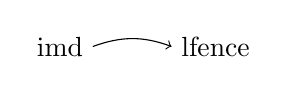
\begin{tikzpicture}
    \node (imd) {\gls{imd}};
    \node[right=1.0 of imd] (lfence) {\gls{lfence}};

    \draw[->] (imd.east) to[bend left=20] (lfence.west);
  \end{tikzpicture}}
  \caption{Compatibility of source-code instrumentations to prevent attacks of individual or multiple SPECTRE-variants.
  Nodes are compilers that perform the respective source-code instrumentation. 
  Edges are directed and represent compatibility of the composition. 
  Tha origin of an edge is the compiler that should be run first, the target of an edge is the compiler that should be run afterwards.}
\end{figure}

\section{Conclusion}

This short paper sketched a real-world application of the compositionality framework for secure compilers as presented in earlier work\MK{cit}. 
While few source-code transformations have been formally proven secure, it is nonetheless interesting to investigate their compatiblity relationships with other transformations on a semantic level, pretending the passes have been proven secure.
Future work considers more source-code instrumentations, not only on just speculation. 
Most interestingly, the authors would like to investigate the compatiblity of common compiler optimisations.

\newpage

%% Bibliography
\bibliography{library}
% \bibliography{./../library}


%% Appendix
%\appendix
%\section{Appendix}

%Text of appendix \ldots

\end{document}
